\title{The Adaptive Multi-scale Simulation Infrastructure - Design and Application}
\author{W.R. Tobin, V.W.L. Chan, M.S. Shephard}
\date{\today}
\documentclass[11pt]{siamltex1213}
\bibliographystyle{siam}

\usepackage{graphicx}
\usepackage{mathtools}
\DeclarePairedDelimiter\ceil{\lceil}{\rceil}
\DeclarePairedDelimiter\floor{\lfloor}{\rfloor}

\begin{document}
\maketitle

\begin{abstract}
\end{abstract}

\section{Note}\label{note}
This article predominantly discusses multi-scale simulations - wherein two or more separate physical scales are involved in the simulation - the discussion is equally applicable to multi-model simulations - wherein two or more numerical or physical models operating on the same domain (possibly with differing discretizations) are involved in the simulation - as well as to simulations which are both.

\section{Introduction}\label{introduction}
\label{single_scale_simulations}
Most physical models and implementations using numerical methods operate at a single scale characteristic to the problem. The scale at which the preponderance of attributes governing the underlying physics being modelled are measured and the resolution of the numerical solution is considered acceptable for the desired accuracy of the simulation.

\label{multi_scale_simulations}
Introduction of influence from scales orders of magnitude removed from the primary scale can take place in several different ways. This influence can be incorporated during the mathematical development of the physical model itself. In this case the multi-scale features are incorporated into the numerical implementation automatically, as a result of their presence in the mathematical model. 

Multi-scale influences can also be incorporated in a more strictly numerical sense, combining physical models operating at different scales referencing and effecting shared physical fields and values \cite{shenoy97} \cite{weinan2003heterogenous}. Numerically multi-scale simulations associate many numerical implementations of single-scale physical models and cause them to interact through passing key physical terms between scales. This scale-coupling will involve up-/down-scaling operations to account for differences in scale dimension, as well as possibly dimensionalizing terms computed in a non-dimensional domain.

In order for a numerically multi-scale approach to be effective the domain at the scale of interest (or engineering scale) must be sufficiently large that conducting the entire simulation with terms and granularity orders of magnitude smaller would make the simulation computationally intractable. Thus some computationally reasonable subset of the engineering scale is assigned tertiary scales to simulate. The precise choice of location of the tertiary simulations is largely dependent on the specific numerical algorithms used to implement the engineering scale simulation. 

Often the subset(s) of the domain associated with the tertiary scale(s) are locations in the engineering domain where the impact of the tertiary scales has the most impact on the engineering scale simulation, in order to leverage the most power from the multi-scale approach.

In the concurrent multi-scale paradigm, all scales are computed simultaneously and the required inter-scale coupling values are provided just-in-time \cite{zeng2010concurrent}.

In the sequential multi-scale paradigm, tertiary scales compute parameters which are converted to quantities of utility to a primary scale. Each scale (though not necessarily each scale-task, representing an individual operation or simulation occurring in a scale) must be processed sequentially \cite{garcia2008sequential} and may be blocked on the completion of the previous scale. This multi-scale model maps intuitively to phased parallel communication models found in the commonly used bulk synchronous parallel abstraction \cite{valiant1990bridging}. 

\subsection{Adaptive Multi-scale Simulation Infrastructure}\label{amsi}
The Adaptive Multi-scale Simulation Infrastructure (amsi) is a set of libraries and tools developed at the Scientific Computation Research Center (SCOREC) at Rensselaer Polytechnic Institute. Amsi is designed to support the implementation and execution of dynamic numerically multi-scale simulations on massively-parallel HPC machines. Currently amsi provides interfaces for describing and managing the execution of individual scales in a multi-scale simulation, for defining and managing the scale-coupling communication required by such simulations, and for planning and enacting scale-sensitive load balancing operations on individual scales in a multi-scale system. 

The interfaces provided by the amsi libraries are intended to facilitate the coupling of functional (possibly legacy) simulation codes already in usage for single-scale problems, in order to avoid development overhead associated with casting a simulation into a set of framework-specific components. The currently implemented interfaces are physics-agnostic, operating only on computational quantities with no model of a term's relation to the mathematical derivation of the multi-scale interaction. Incorporation of meta-information and services targeted toward specific multi-scale physical couplings represents a desirable extension of the amsi libraries, constituting a rich area of future work.

Amsi operates by maintaining a set of minimal simulation metadata in order to model various quantities of interest during simulation execution. A decentralized approach toward control is taken; dynamic control decisions are made and implemented at runtime during collective operations. In order to avoid the introduction of unnecessary parallel barriers into the code, amsi control decisions are only made during operations which are already collective over the set of processes effected by a given control decision.

\subsection{Novelty} %rename
Frameworks and runtime systems have been developed which are intended for the development of specific multi-scale problems \cite{parker2006component} \cite{chopard2011framework} \cite{} and these frameworks have in some cases been expanded to facilitate the implementation of additional multi-scale problems \cite{berzins2010uintah}.

These systems suffer from the requirement that an application developer must cast the problem of interest into a set of predefined components (interfaces, tasks, etc.) or high-level modelling language in order to take full advantage of such frameworks. Leveraging a component-based design is valuable from a software engineering perspective, but also introduces new complexities involved in defining the set of components and how they interoperate in the framework shifting some complexity up a level of abstraction. The core features of amsi used for multi-scale simulation management and communication are provided with no requirements of adherence to a specific component definition.

simulation flow control is determined solely by the runtime system. A framework may also limit specific features of the numerical implementation to those provided by the framework. Domain discretization models and associated adaptive processes -- structured and unstructured meshing and associated refinement algorithms, particle-in-cell methods, etc. -- convergence algorithms for both the minimization of the relevant residuals (Newton-Raphson, etc.) as well as iterative solution of the resulting linear system (KSP, GMRES, ILU, etc.). Amsi supplies several numerical components consisting of an adaptive finite element system, linear algebraic solver, and nonlinear convergence operators available as both simple C++ class interface definitions, as well as implementations built on top of other software supplied by SCOREC \cite{core} and the PETSc linear algebraic solver \cite{petsc-web-page} \cite{petsc-user-ref} \cite{petsc-efficient}. Usage of the supplied numerical components is not required to make use of the multi-scale meta-modeling, communication, dynamic instantiation, and scale-sensitive load balancing facilities supplied by amsi.

Implementing required numerical operations inside an existing framework is of course possible, though it may prove an additional -- undesirable overhead for an application programmer interested only in utilizing the multi-scale framework to implement a simulation, rather than implementing the various numerical operations often optimized in widely available packages and libraries.

\label{amsi_scales}
A configuration file is supplied during command invocation containing the initial configuration of the process sets and their assignment to individual scales, as well as declaring the coupling between scales in the simulation. The deceleration of a scale and the initialization of the process set associated with the scale are considered a single atomic operation in the current implementation.

Process sets are mathematical sets of MPI ranks implemented so as to take advantage of any mathematical conveniences to minimize explicit storage whenever possible. Process sets are required to be non-overlapping in order for amsi control mechanisms to operate correctly. Ongoing developments are targeted at removing this requirement to allow a richer set of dynamic control options and increase overall utilization in the case of coupled scales blocking on one another. 

Deceleration of a coupling relation between two scales is required if any communication between the scales is to occur during the simulation (through the amsi libraries), as the coupling deceleration during simulation initialization is used to instantiate data structures specific to scale-coupling operations. This limits memory overhead by not allocating space for unneeded coupling operations.

Scales are declared to be related if some quantities of interest (such as physical tensor field values) are transmitted between them for scale-coupling. This coupling relationship is assumed to be asymmetric, thus if scale A is related to scale B, scale B is not implicitly related to scale A, though this may be separately declared. For brevity this may be written as A~B for A is coupled to B.

While the primary scale (the scale associated with producing the solution for the overall simulation) is often thought of as controlling the tertiary scales in terms of dynamic instantiation, this is not assumed in the amsi implementation. Any scale is capable of informing the process set associated with a coupled scale of the addition or deletion of individual scale-tasks. At present it is dependent on the developer to implement the capability of a scale to accept additional scale-tasks, though algorithms and hooks for developer-designed distribution algorithms are supplied to ease the implementation.

\label{amsi_communication}
Scale-coupling communication is guided by data distributions and communication patterns. A data distribution is a representation of individual units of scale-coupling data distributed across a single scale-task. The format of the coupling data is arbitrary (so long as it can be serialized and provided for use by MPI communication primitives). A data distribution represents the smallest unit of data important to the scale-coupling communication, which is necessarily distinct for various multi-scale use cases. 

All communication and planning operations in the amsi libraries use an implicit local numbering for data distribution terms, the index associated with the term in a local serialized buffer. At present an application developer must implement up-/down-scaling operations required for their particular multi-scale use case, hooks will be provided in a future release to automate application of such operations during scale-coupling.

\label{amsi_load_balancing}
If a local installation of the Zoltan \cite{ZoltanOverviewArticle2002} \cite{ZoltanIsorropiaOverview2012} load balancing library is available, the load balancing planning algorithms of Zoltan can be used underlying the scale-sensitive load balancing planning of amsi. A minimal set of load-balancing algorithms are provided with amsi. Since there is no general solution to the dynamic load balancing problem any set of provided load-balancing algorithms will prove insufficient for some use case. Thus amsi provides users with the ability to create and register their own load-balancing algorithms specific to the requirements of a given numerical implementation.

Due to the necessity of retaining inter-scale linkages through the load-balancing processes, the actual data migration undertaken to implement a specific load balancing plan is typically conducted internally by the amsi system which is provided with buffers of data being load-balanced by each process on the appropriate scale. However, in order to maintain usability in more general situations, it is also possible to simply inform the amsi system that the current load-balancing plan has already been accomplished by user-implemented data migration. This functionality combined with the ability to use user-designed load-balance planning algorithms allows amsi to work with entirely external load-balancing libraries and algorithms, allowing scale-sensitive load-balancing to be used even when a specific multi-scale use case falls outside the bounds of capabilities built into the system.

\subsection{Soft Tissue Simulation}\label{biotissue}
The Biotissue code is a multi-scale simulation of soft organic tissues, consisting of an engineering-scale simulation using the finite element method, and a micro-scale quasistatics force-balance simulation. The Cauchy Momentum Balance Equation for a body in static equilibrium is used as the governing equation for the global simulation. Specific quantities needed to compute the elemental tangent stiffness matrices are instead supplied by the micro-scale force-balance simulations, which occur at each numerical integration point in the engineering-scale mesh \ref{biotissue_hierarchy}. 

\begin{figure}
  \begin{center}
    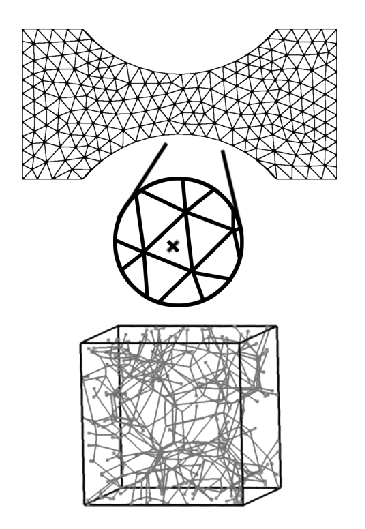
\includegraphics[height=2in]{biotissue_visual_hierarchy.eps}
  \end{center}
  \caption{\small biotissue multi-scale problem}
  \label{biotissue_hierarchy}
\end{figure}

The incremental displacements (deltas generated by the previous Newton-Raphson iteration) on each engineering-scale finite element node are used to distort the a dimensionless representative volume element (RVE) through a dimensionalized abstraction of the RVE embedded in the engineering domain and an associated displacement mapping term $\frac{d\mathbf{RVE}}{d\mathbf{FE}}$, the first order relation between the incremental displacement of an RVE with respect to the displacement of the associated mesh element. This results in each micro-scale node being displaced. Each RVE is a dimensionless unit cube containing a connected collagen fiber network, for the present results the fibers are implemented as truss elements and their distribution is generated using Delauney triangulation. The micro-scale boundary condition necessitates that the force exerted by each fiber network node located on the boundary of the RVE be zero. The micro-scale global Jacobian is formulated along with the force vector, wherein the boundary condition is enforced by setting specific rows of the force vector associated with boundary nodes to zero. 

Another Newton-Raphson iterative process occurs at micro-scale to converge to the set of displacements resulting in force equilibrium for all the fibers within the fiber network constituting the RVE. After a micro-scale simulation converges to a solution, the Jacobian and force vector are then evaluated again at the solution position, the force exerted along the boundary of the RVE is summed for each of the principal and shear components of a stress tensor, which is then dimensionalized and sent back to the engineering-scale for use in the elemental tangent stiffness matrix formulation. More detail into the derivation of this multi-scale system can be found in \cite{stylianopoulos2008thesis} \cite{agoram2001coupled} \cite{stylianopoulos2007multiscale} . Discussion of the dimensionalization of the dimensionless force terms produced by each fiber network can be found in \cite{stylianopoulos2007volume} \cite{chandran2007deterministic}.

%Typically in the displacement-based finite element method, a constitutive model depending on some set of material properties is derived from a set of governing physical partial differential equations. In the case of the Biotissue multi-scale code, the constitutive model governing the systemic response to the boundary conditions is supplemented by the micro-scale force-balance simulation. The Newton-Raphson method is used to iterate to the solution for a particular loading state, and at each Newton iteration the global tangent stiffness matrix is assembled from elemental systems generated from each element in the engineering-scale mesh. In typically FEM the elemental system is derived from the governing material model used for the specific type of material being simulated; for the Biotissue code the necessary values are instead provided as 

Thus the simulation as a whole is essentially doubly nonlinear, as during each engineering-scale Newton iteration every micro-scale RVE must undergo a full Newton-Raphson convergence process. 

\section{Results}\label{results}
The biotissue simulation was run on the AMOS BG/Q machine housed at the CCI facilities. Both strong and weak scaling studies were conducted up to an eighth of the total machine core count, or 16384 cores. The ratio of macro-scale to micro-scale assigned processes was held near 1:128, though the total core count was kept as an integer power of 2 in order for the SLURM job scheduler to submit the jobs to the compute nodes in a timely manner. The precise calculation used to determine macro and micro ratio is given by 
$$ 
num_macro = N 
num_cores = N*128
num_micro = num_cores - N
$$
thus as the number of cores assigned to the macro-scale computation scales, the ratio approaches 1:128. 

Separate timings were taken for various sections of the simulation code, isolating the micro-scale computation, macro-scale linear system assembly and calculation of elemental linear systems, and macro-scale linear system solution. In addition, the time for spent in the amsi subroutines for communication was also measured. Thus the behavior of each section of the code is independently evaluated in our scaling study, as well as the overall execution time.

Weak scaling.

Strong scaling.

Amsi-specific results of some sort...?

\section{Future Work}\label{future_work}

Work on scale-balancing is ongoing for the biotissue test problem. Using this work as a basis, a set of algorithms to provide support for more general scale-balancing operations will be developed and packaged into amsi.

Scale-sensitive load-balancing operations have been developed for the biotissue multi-scale test problem. Unfortunately the problem does not exhibit load persistence in the current parallel task discretization, so an alternative parallel discretization such as overdecomposition with work-stealing to enforce more local balancing operations and occasional global balancing operations is being explored.

Embedded fiber-matrix RVEs separately parallelized and incorporated into multi-scale model, used at most error-sensitive locations \cite{lake2012mechanics} \cite{zhang2013cross} \cite{zhang2013coupled}.

\bibliography{citations}

\end{document}
